% Options for packages loaded elsewhere
\PassOptionsToPackage{unicode}{hyperref}
\PassOptionsToPackage{hyphens}{url}
%
\documentclass[
]{article}
\usepackage{amsmath,amssymb}
\usepackage{iftex}
\ifPDFTeX
  \usepackage[T1]{fontenc}
  \usepackage[utf8]{inputenc}
  \usepackage{textcomp} % provide euro and other symbols
\else % if luatex or xetex
  \usepackage{unicode-math} % this also loads fontspec
  \defaultfontfeatures{Scale=MatchLowercase}
  \defaultfontfeatures[\rmfamily]{Ligatures=TeX,Scale=1}
\fi
\usepackage{lmodern}
\ifPDFTeX\else
  % xetex/luatex font selection
\fi
% Use upquote if available, for straight quotes in verbatim environments
\IfFileExists{upquote.sty}{\usepackage{upquote}}{}
\IfFileExists{microtype.sty}{% use microtype if available
  \usepackage[]{microtype}
  \UseMicrotypeSet[protrusion]{basicmath} % disable protrusion for tt fonts
}{}
\makeatletter
\@ifundefined{KOMAClassName}{% if non-KOMA class
  \IfFileExists{parskip.sty}{%
    \usepackage{parskip}
  }{% else
    \setlength{\parindent}{0pt}
    \setlength{\parskip}{6pt plus 2pt minus 1pt}}
}{% if KOMA class
  \KOMAoptions{parskip=half}}
\makeatother
\usepackage{xcolor}
\usepackage[margin=1in]{geometry}
\usepackage{color}
\usepackage{fancyvrb}
\newcommand{\VerbBar}{|}
\newcommand{\VERB}{\Verb[commandchars=\\\{\}]}
\DefineVerbatimEnvironment{Highlighting}{Verbatim}{commandchars=\\\{\}}
% Add ',fontsize=\small' for more characters per line
\usepackage{framed}
\definecolor{shadecolor}{RGB}{248,248,248}
\newenvironment{Shaded}{\begin{snugshade}}{\end{snugshade}}
\newcommand{\AlertTok}[1]{\textcolor[rgb]{0.94,0.16,0.16}{#1}}
\newcommand{\AnnotationTok}[1]{\textcolor[rgb]{0.56,0.35,0.01}{\textbf{\textit{#1}}}}
\newcommand{\AttributeTok}[1]{\textcolor[rgb]{0.13,0.29,0.53}{#1}}
\newcommand{\BaseNTok}[1]{\textcolor[rgb]{0.00,0.00,0.81}{#1}}
\newcommand{\BuiltInTok}[1]{#1}
\newcommand{\CharTok}[1]{\textcolor[rgb]{0.31,0.60,0.02}{#1}}
\newcommand{\CommentTok}[1]{\textcolor[rgb]{0.56,0.35,0.01}{\textit{#1}}}
\newcommand{\CommentVarTok}[1]{\textcolor[rgb]{0.56,0.35,0.01}{\textbf{\textit{#1}}}}
\newcommand{\ConstantTok}[1]{\textcolor[rgb]{0.56,0.35,0.01}{#1}}
\newcommand{\ControlFlowTok}[1]{\textcolor[rgb]{0.13,0.29,0.53}{\textbf{#1}}}
\newcommand{\DataTypeTok}[1]{\textcolor[rgb]{0.13,0.29,0.53}{#1}}
\newcommand{\DecValTok}[1]{\textcolor[rgb]{0.00,0.00,0.81}{#1}}
\newcommand{\DocumentationTok}[1]{\textcolor[rgb]{0.56,0.35,0.01}{\textbf{\textit{#1}}}}
\newcommand{\ErrorTok}[1]{\textcolor[rgb]{0.64,0.00,0.00}{\textbf{#1}}}
\newcommand{\ExtensionTok}[1]{#1}
\newcommand{\FloatTok}[1]{\textcolor[rgb]{0.00,0.00,0.81}{#1}}
\newcommand{\FunctionTok}[1]{\textcolor[rgb]{0.13,0.29,0.53}{\textbf{#1}}}
\newcommand{\ImportTok}[1]{#1}
\newcommand{\InformationTok}[1]{\textcolor[rgb]{0.56,0.35,0.01}{\textbf{\textit{#1}}}}
\newcommand{\KeywordTok}[1]{\textcolor[rgb]{0.13,0.29,0.53}{\textbf{#1}}}
\newcommand{\NormalTok}[1]{#1}
\newcommand{\OperatorTok}[1]{\textcolor[rgb]{0.81,0.36,0.00}{\textbf{#1}}}
\newcommand{\OtherTok}[1]{\textcolor[rgb]{0.56,0.35,0.01}{#1}}
\newcommand{\PreprocessorTok}[1]{\textcolor[rgb]{0.56,0.35,0.01}{\textit{#1}}}
\newcommand{\RegionMarkerTok}[1]{#1}
\newcommand{\SpecialCharTok}[1]{\textcolor[rgb]{0.81,0.36,0.00}{\textbf{#1}}}
\newcommand{\SpecialStringTok}[1]{\textcolor[rgb]{0.31,0.60,0.02}{#1}}
\newcommand{\StringTok}[1]{\textcolor[rgb]{0.31,0.60,0.02}{#1}}
\newcommand{\VariableTok}[1]{\textcolor[rgb]{0.00,0.00,0.00}{#1}}
\newcommand{\VerbatimStringTok}[1]{\textcolor[rgb]{0.31,0.60,0.02}{#1}}
\newcommand{\WarningTok}[1]{\textcolor[rgb]{0.56,0.35,0.01}{\textbf{\textit{#1}}}}
\usepackage{graphicx}
\makeatletter
\def\maxwidth{\ifdim\Gin@nat@width>\linewidth\linewidth\else\Gin@nat@width\fi}
\def\maxheight{\ifdim\Gin@nat@height>\textheight\textheight\else\Gin@nat@height\fi}
\makeatother
% Scale images if necessary, so that they will not overflow the page
% margins by default, and it is still possible to overwrite the defaults
% using explicit options in \includegraphics[width, height, ...]{}
\setkeys{Gin}{width=\maxwidth,height=\maxheight,keepaspectratio}
% Set default figure placement to htbp
\makeatletter
\def\fps@figure{htbp}
\makeatother
\setlength{\emergencystretch}{3em} % prevent overfull lines
\providecommand{\tightlist}{%
  \setlength{\itemsep}{0pt}\setlength{\parskip}{0pt}}
\setcounter{secnumdepth}{-\maxdimen} % remove section numbering
\usepackage{booktabs}
\usepackage{longtable}
\usepackage{array}
\usepackage{multirow}
\usepackage{wrapfig}
\usepackage{float}
\usepackage{colortbl}
\usepackage{pdflscape}
\usepackage{tabu}
\usepackage{threeparttable}
\usepackage{threeparttablex}
\usepackage[normalem]{ulem}
\usepackage{makecell}
\usepackage{xcolor}
\ifLuaTeX
  \usepackage{selnolig}  % disable illegal ligatures
\fi
\IfFileExists{bookmark.sty}{\usepackage{bookmark}}{\usepackage{hyperref}}
\IfFileExists{xurl.sty}{\usepackage{xurl}}{} % add URL line breaks if available
\urlstyle{same}
\hypersetup{
  pdftitle={Kaufman\_McNeill\_ENV797\_Project},
  pdfauthor={Emma Kaufman and Jenn McNeill},
  hidelinks,
  pdfcreator={LaTeX via pandoc}}

\title{Kaufman\_McNeill\_ENV797\_Project}
\author{Emma Kaufman and Jenn McNeill}
\date{2024-04-10}

\begin{document}
\maketitle

\begin{Shaded}
\begin{Highlighting}[]
\FunctionTok{library}\NormalTok{(lubridate)}
\end{Highlighting}
\end{Shaded}

\begin{verbatim}
## 
## Attaching package: 'lubridate'
\end{verbatim}

\begin{verbatim}
## The following objects are masked from 'package:base':
## 
##     date, intersect, setdiff, union
\end{verbatim}

\begin{Shaded}
\begin{Highlighting}[]
\FunctionTok{library}\NormalTok{(ggplot2)}
\FunctionTok{library}\NormalTok{(forecast)  }
\end{Highlighting}
\end{Shaded}

\begin{verbatim}
## Registered S3 method overwritten by 'quantmod':
##   method            from
##   as.zoo.data.frame zoo
\end{verbatim}

\begin{Shaded}
\begin{Highlighting}[]
\FunctionTok{library}\NormalTok{(Kendall)}
\FunctionTok{library}\NormalTok{(tseries)}
\FunctionTok{library}\NormalTok{(outliers)}
\FunctionTok{library}\NormalTok{(tidyverse)}
\end{Highlighting}
\end{Shaded}

\begin{verbatim}
## -- Attaching core tidyverse packages ------------------------ tidyverse 2.0.0 --
## v dplyr   1.1.3     v stringr 1.5.0
## v forcats 1.0.0     v tibble  3.2.1
## v purrr   1.0.2     v tidyr   1.3.0
## v readr   2.1.4
\end{verbatim}

\begin{verbatim}
## -- Conflicts ------------------------------------------ tidyverse_conflicts() --
## x dplyr::filter() masks stats::filter()
## x dplyr::lag()    masks stats::lag()
## i Use the conflicted package (<http://conflicted.r-lib.org/>) to force all conflicts to become errors
\end{verbatim}

\begin{Shaded}
\begin{Highlighting}[]
\FunctionTok{library}\NormalTok{(smooth)}
\end{Highlighting}
\end{Shaded}

\begin{verbatim}
## Loading required package: greybox
## Package "greybox", v2.0.0 loaded.
## 
## 
## Attaching package: 'greybox'
## 
## The following object is masked from 'package:tidyr':
## 
##     spread
## 
## The following object is masked from 'package:lubridate':
## 
##     hm
## 
## This is package "smooth", v4.0.0
## If you want to know more about the smooth package and forecasting, you can visit my website: https://forecasting.svetunkov.ru/
\end{verbatim}

\begin{Shaded}
\begin{Highlighting}[]
\FunctionTok{library}\NormalTok{(dplyr)}
\FunctionTok{library}\NormalTok{(cowplot)}
\end{Highlighting}
\end{Shaded}

\begin{verbatim}
## 
## Attaching package: 'cowplot'
## 
## The following object is masked from 'package:lubridate':
## 
##     stamp
\end{verbatim}

\begin{Shaded}
\begin{Highlighting}[]
\FunctionTok{library}\NormalTok{(corrplot)}
\end{Highlighting}
\end{Shaded}

\begin{verbatim}
## corrplot 0.92 loaded
\end{verbatim}

\begin{Shaded}
\begin{Highlighting}[]
\FunctionTok{library}\NormalTok{(kableExtra)}
\end{Highlighting}
\end{Shaded}

\begin{verbatim}
## 
## Attaching package: 'kableExtra'
## 
## The following object is masked from 'package:dplyr':
## 
##     group_rows
\end{verbatim}

Provide information on how the dataset for this analysis were collected
(source), the data contained in the dataset (format). Describe how you
wrangled/processed your dataset to get the time series object.

Add a table that summarizes your data structure (variables, units,
ranges and/or central tendencies, data source if multiple are used,
etc.). This table should inserted as a \texttt{kable} function in an R
chunk. Just show the first 10 rows of your data. Do not include the code
used to generate your table.

The dataset for this analysis was collected from the
\href{https://www.kaggle.com/c/acea-water-prediction/data}{Acea Group
Smart Water Analytics Competition on Kaggle}. The Acea Group is an
Italian utility operator that develops and maintains water networks for
9 million constituents. As a utility operator, they are concerned with
preserving waterbodies and thus forecasting the water levels at the
sources where they get their water. The competition included nine
different datasets that represented water springs, lakes, rivers, or
aquifers and had unique attributes and characteristics. For our final
project, we decided to focus our time series modeling and forecasting on
the Auser Aquifer. Our objective is to predict the amount of water in
the Auser Aquifer by modeling the depth to groundwater and
simultaneously evaluate how other variables such as rainfall,
temperature, and treatment plant volume may impact our prediction.

The dataset for the Auser Aquifer includes daily depth to groundwater
measurements (in meters) from five different wells across the north and
south sectors. Wells SAL, PAG, CoS, and DIEC represent the north while
Well LT2 represents the south. We also have daily temperatyre data at
four sites, daily rainfall data at ten sites, and daily volume data from
five different water treatment facilities.

\begin{Shaded}
\begin{Highlighting}[]
\FunctionTok{head}\NormalTok{(auser\_raw)}
\end{Highlighting}
\end{Shaded}

\begin{verbatim}
##         Date Rainfall_Gallicano Rainfall_Pontetetto Rainfall_Monte_Serra
## 1 1998-03-05                 NA                  NA                   NA
## 2 1998-03-06                 NA                  NA                   NA
## 3 1998-03-07                 NA                  NA                   NA
## 4 1998-03-08                 NA                  NA                   NA
## 5 1998-03-09                 NA                  NA                   NA
## 6 1998-03-10                 NA                  NA                   NA
##   Rainfall_Orentano Rainfall_Borgo_a_Mozzano Rainfall_Piaggione
## 1                NA                       NA                 NA
## 2                NA                       NA                 NA
## 3                NA                       NA                 NA
## 4                NA                       NA                 NA
## 5                NA                       NA                 NA
## 6                NA                       NA                 NA
##   Rainfall_Calavorno Rainfall_Croce_Arcana
## 1                 NA                    NA
## 2                 NA                    NA
## 3                 NA                    NA
## 4                 NA                    NA
## 5                 NA                    NA
## 6                 NA                    NA
##   Rainfall_Tereglio_Coreglia_Antelminelli Rainfall_Fabbriche_di_Vallico
## 1                                      NA                            NA
## 2                                      NA                            NA
## 3                                      NA                            NA
## 4                                      NA                            NA
## 5                                      NA                            NA
## 6                                      NA                            NA
##   Depth_to_Groundwater_LT2 Depth_to_Groundwater_SAL Depth_to_Groundwater_PAG
## 1                       NA                       NA                       NA
## 2                       NA                       NA                       NA
## 3                       NA                       NA                       NA
## 4                       NA                       NA                       NA
## 5                       NA                       NA                       NA
## 6                       NA                       NA                       NA
##   Depth_to_Groundwater_CoS Depth_to_Groundwater_DIEC Temperature_Orentano
## 1                       NA                        NA                    0
## 2                       NA                        NA                    0
## 3                       NA                        NA                    0
## 4                       NA                        NA                    0
## 5                       NA                        NA                    0
## 6                       NA                        NA                    0
##   Temperature_Monte_Serra Temperature_Ponte_a_Moriano
## 1                    0.00                           0
## 2                    0.00                           0
## 3                    9.20                           0
## 4                   11.40                           0
## 5                   11.40                           0
## 6                    7.95                           0
##   Temperature_Lucca_Orto_Botanico Volume_POL Volume_CC1 Volume_CC2 Volume_CSA
## 1                            0.00         NA         NA         NA         NA
## 2                           10.05         NA         NA         NA         NA
## 3                           10.00         NA         NA         NA         NA
## 4                           13.85         NA         NA         NA         NA
## 5                           12.85         NA         NA         NA         NA
## 6                            6.50         NA         NA         NA         NA
##   Volume_CSAL Hydrometry_Monte_S_Quirico Hydrometry_Piaggione
## 1          NA                         NA                   NA
## 2          NA                         NA                   NA
## 3          NA                         NA                   NA
## 4          NA                         NA                   NA
## 5          NA                         NA                   NA
## 6          NA                         NA                   NA
\end{verbatim}

\begin{Shaded}
\begin{Highlighting}[]
\NormalTok{data\_information }\OtherTok{\textless{}{-}} \FunctionTok{data.frame}\NormalTok{(}
  \AttributeTok{Source =}\NormalTok{ (}\StringTok{"Acea Group Smart Water Analytics Competition on Kaggle"}\NormalTok{),}
  \AttributeTok{Variables =} \FunctionTok{c}\NormalTok{(}\StringTok{"Date, Rainfall\_Gallicano, Rainfall\_Pontetetto, Rainfall\_Monte\_Serra,}
\StringTok{                Rainfall\_Orentano, Rainfall\_Borgo\_a\_Mozzano, Rainfall\_Piaggione,}
\StringTok{                Rainfall\_Calavorno, Rainfall\_Croce\_Arcana, }
\StringTok{                Rainfall\_Tereglio\_Coreglia\_Antelminelli, Rainfall\_Fabbriche\_di\_Vallico, }
\StringTok{                Depth\_to\_Groundwater\_LT2, Depth\_to\_Groundwater\_SAL, Depth\_to\_Groundwater\_PAG, }
\StringTok{                Depth\_to\_Groundwater\_CoS, Depth\_to\_Groundwater\_DIEC, Temperature\_Orentano, }
\StringTok{                Temperature\_Monte\_Serra, Temperature\_Ponte\_a\_Moriano, }
\StringTok{                Temperature\_Lucca\_Orto\_Botanico, Volume\_POL, Volume\_CC1, Volume\_CC2, }
\StringTok{                Volume\_CSA, Volume\_CSAL, Hydrometry\_Monte\_S\_Quirico, Hydrometry\_Piaggione"}\NormalTok{),}
  \AttributeTok{Units =} \FunctionTok{c}\NormalTok{(}\StringTok{"Date: Year, Month, Date format, Rainfall: millimeters, Depth to Groundwater: }
\StringTok{                meters, Temperature: Degrees Celcius, Volume: figure this out, Hydrometry:}
\StringTok{                figure this out"}\NormalTok{))}

\FunctionTok{kbl}\NormalTok{(data\_information, }\AttributeTok{caption=}\StringTok{"Data Source and Structure"}\NormalTok{) }\SpecialCharTok{\%\textgreater{}\%} 
  \FunctionTok{kable\_styling}\NormalTok{(}\AttributeTok{full\_width =} \ConstantTok{FALSE}\NormalTok{, }
                \AttributeTok{position =} \StringTok{"center"}\NormalTok{,}
                \AttributeTok{latex\_options =} \StringTok{"hold\_position"}\NormalTok{)}
\end{Highlighting}
\end{Shaded}

\begin{table}[!h]

\caption{\label{tab:unnamed-chunk-2}Data Source and Structure}
\centering
\begin{tabular}[t]{l|l|l}
\hline
Source & Variables & Units\\
\hline
Acea Group Smart Water Analytics Competition on Kaggle & Date, Rainfall\_Gallicano, Rainfall\_Pontetetto, Rainfall\_Monte\_Serra,
                Rainfall\_Orentano, Rainfall\_Borgo\_a\_Mozzano, Rainfall\_Piaggione,
                Rainfall\_Calavorno, Rainfall\_Croce\_Arcana, 
                Rainfall\_Tereglio\_Coreglia\_Antelminelli, Rainfall\_Fabbriche\_di\_Vallico, 
                Depth\_to\_Groundwater\_LT2, Depth\_to\_Groundwater\_SAL, Depth\_to\_Groundwater\_PAG, 
                Depth\_to\_Groundwater\_CoS, Depth\_to\_Groundwater\_DIEC, Temperature\_Orentano, 
                Temperature\_Monte\_Serra, Temperature\_Ponte\_a\_Moriano, 
                Temperature\_Lucca\_Orto\_Botanico, Volume\_POL, Volume\_CC1, Volume\_CC2, 
                Volume\_CSA, Volume\_CSAL, Hydrometry\_Monte\_S\_Quirico, Hydrometry\_Piaggione & Date: Year, Month, Date format, Rainfall: millimeters, Depth to Groundwater: 
                meters, Temperature: Degrees Celcius, Volume: figure this out, Hydrometry:
                figure this out\\
\hline
\end{tabular}
\end{table}

The first obstacle with wrangling our data came when we realized that
the data for each variable started at a different date. We found this
issue by plotting the five depth to groundwater lines and seeing a large
lag before the data started, NA values within each series, and a few
random ``zero'' values that we assumed to be errors. To rectify this
issue, we converted all ``zero'' values to NA, found the start date for
each well's data, and then converted each well's data into a time series
object. When we plotted these five time series together, we still had
gaps of NA data. We ran the tsclean function to fill in the gaps of
missing data with interpolated values and then had five clean series
with no data gaps.

\begin{Shaded}
\begin{Highlighting}[]
\CommentTok{\#create a time series object of the values for depth to groundwater for each well}
\CommentTok{\#start the time series at the same unique first day of data as above}
\NormalTok{ts\_LT2 }\OtherTok{\textless{}{-}} \FunctionTok{ts}\NormalTok{(LT2\_depth[,}\DecValTok{2}\NormalTok{],}\AttributeTok{start=}\FunctionTok{c}\NormalTok{(}\DecValTok{2006}\NormalTok{,}\DecValTok{01}\NormalTok{,}\DecValTok{01}\NormalTok{), }\AttributeTok{frequency=}\DecValTok{365}\NormalTok{)}
\NormalTok{ts\_SAL }\OtherTok{\textless{}{-}} \FunctionTok{ts}\NormalTok{(SAL\_depth[,}\DecValTok{2}\NormalTok{],}\AttributeTok{start=}\FunctionTok{c}\NormalTok{(}\DecValTok{2007}\NormalTok{,}\DecValTok{04}\NormalTok{,}\DecValTok{06}\NormalTok{), }\AttributeTok{frequency=}\DecValTok{365}\NormalTok{)}
\NormalTok{ts\_PAG }\OtherTok{\textless{}{-}} \FunctionTok{ts}\NormalTok{(PAG\_depth[,}\DecValTok{2}\NormalTok{],}\AttributeTok{start=}\FunctionTok{c}\NormalTok{(}\DecValTok{2009}\NormalTok{,}\DecValTok{01}\NormalTok{,}\DecValTok{01}\NormalTok{), }\AttributeTok{frequency=}\DecValTok{365}\NormalTok{)}
\NormalTok{ts\_CoS }\OtherTok{\textless{}{-}} \FunctionTok{ts}\NormalTok{(CoS\_depth[,}\DecValTok{2}\NormalTok{], }\AttributeTok{start =} \FunctionTok{c}\NormalTok{(}\DecValTok{2008}\NormalTok{,}\DecValTok{01}\NormalTok{,}\DecValTok{25}\NormalTok{), }\AttributeTok{frequency=} \DecValTok{365}\NormalTok{)}
\NormalTok{ts\_DIEC }\OtherTok{\textless{}{-}} \FunctionTok{ts}\NormalTok{(DIEC\_depth[,}\DecValTok{2}\NormalTok{], }\AttributeTok{start =} \FunctionTok{c}\NormalTok{(}\DecValTok{2011}\NormalTok{,}\DecValTok{01}\NormalTok{,}\DecValTok{02}\NormalTok{), }\AttributeTok{frequency=} \DecValTok{365}\NormalTok{)}

\CommentTok{\#plot all time series together}
\FunctionTok{autoplot}\NormalTok{(ts\_LT2, }\AttributeTok{series =} \StringTok{"LT2"}\NormalTok{)}\SpecialCharTok{+}
  \FunctionTok{autolayer}\NormalTok{(ts\_SAL, }\AttributeTok{series =} \StringTok{"SAL"}\NormalTok{)}\SpecialCharTok{+}
  \FunctionTok{autolayer}\NormalTok{(ts\_PAG, }\AttributeTok{series =} \StringTok{"PAG"}\NormalTok{)}\SpecialCharTok{+}
  \FunctionTok{autolayer}\NormalTok{(ts\_CoS, }\AttributeTok{series =} \StringTok{"CoS"}\NormalTok{)}\SpecialCharTok{+}
  \FunctionTok{autolayer}\NormalTok{(ts\_DIEC, }\AttributeTok{series =} \StringTok{"DIEC"}\NormalTok{)}\SpecialCharTok{+}
  \FunctionTok{labs}\NormalTok{(}\AttributeTok{x =} \StringTok{"Year"}\NormalTok{, }\AttributeTok{y =} \StringTok{"Depth to Groundwater (m)"}\NormalTok{, }\AttributeTok{color =} \StringTok{"Well"}\NormalTok{)}\SpecialCharTok{+}
  \FunctionTok{theme\_light}\NormalTok{()}\SpecialCharTok{+}
  \FunctionTok{ggtitle}\NormalTok{(}\StringTok{"Time Series of Depth to Groundwater at Each Well"}\NormalTok{)}\SpecialCharTok{+}
  \FunctionTok{scale\_x\_continuous}\NormalTok{(}\AttributeTok{name =} \StringTok{"Year"}\NormalTok{, }\AttributeTok{breaks =} \FunctionTok{seq}\NormalTok{(}\AttributeTok{from=}\DecValTok{2006}\NormalTok{, }\AttributeTok{to=}\DecValTok{2022}\NormalTok{, }\AttributeTok{by=}\DecValTok{2}\NormalTok{))}\SpecialCharTok{+}
  \FunctionTok{scale\_y\_continuous}\NormalTok{(}\AttributeTok{name =} \StringTok{"Depth to Groundwater (m)"}\NormalTok{, }
                     \AttributeTok{breaks =} \FunctionTok{seq}\NormalTok{(}\AttributeTok{from=}\SpecialCharTok{{-}}\DecValTok{16}\NormalTok{, }\AttributeTok{to=}\DecValTok{0}\NormalTok{, }\AttributeTok{by=}\DecValTok{2}\NormalTok{))}
\end{Highlighting}
\end{Shaded}

\begin{verbatim}
## Scale for x is already present.
## Adding another scale for x, which will replace the existing scale.
\end{verbatim}

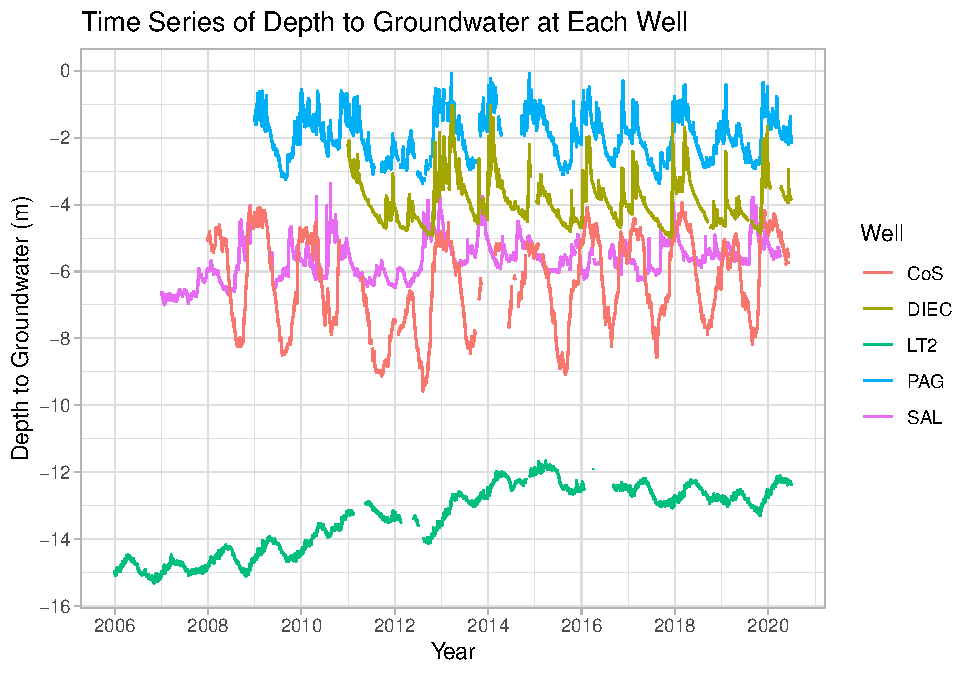
\includegraphics{Kaufman_McNeill_ENV797_Project_files/figure-latex/unnamed-chunk-3-1.pdf}

\begin{Shaded}
\begin{Highlighting}[]
\CommentTok{\#run the clean function on each time series to replace NAs}
\NormalTok{ts\_LT2\_clean }\OtherTok{\textless{}{-}} \FunctionTok{tsclean}\NormalTok{(ts\_LT2)}
\NormalTok{ts\_SAL\_clean }\OtherTok{\textless{}{-}} \FunctionTok{tsclean}\NormalTok{(ts\_SAL)}
\NormalTok{ts\_PAG\_clean }\OtherTok{\textless{}{-}} \FunctionTok{tsclean}\NormalTok{(ts\_PAG)}
\NormalTok{ts\_CoS\_clean }\OtherTok{\textless{}{-}} \FunctionTok{tsclean}\NormalTok{(ts\_CoS)}
\NormalTok{ts\_DIEC\_clean }\OtherTok{\textless{}{-}} \FunctionTok{tsclean}\NormalTok{(ts\_DIEC)}

\CommentTok{\#plot all cleaned time series together}
\FunctionTok{autoplot}\NormalTok{(ts\_LT2\_clean, }\AttributeTok{series =} \StringTok{"LT2"}\NormalTok{)}\SpecialCharTok{+}
  \FunctionTok{autolayer}\NormalTok{(ts\_SAL\_clean, }\AttributeTok{series =} \StringTok{"SAL"}\NormalTok{)}\SpecialCharTok{+}
  \FunctionTok{autolayer}\NormalTok{(ts\_PAG\_clean, }\AttributeTok{series =} \StringTok{"PAG"}\NormalTok{)}\SpecialCharTok{+}
  \FunctionTok{autolayer}\NormalTok{(ts\_CoS\_clean, }\AttributeTok{series =} \StringTok{"CoS"}\NormalTok{)}\SpecialCharTok{+}
  \FunctionTok{autolayer}\NormalTok{(ts\_DIEC\_clean, }\AttributeTok{series =} \StringTok{"DIEC"}\NormalTok{)}\SpecialCharTok{+}
  \FunctionTok{labs}\NormalTok{(}\AttributeTok{x =} \StringTok{"Year"}\NormalTok{, }\AttributeTok{y =} \StringTok{"Depth to Groundwater (m)"}\NormalTok{, }\AttributeTok{color =} \StringTok{"Well"}\NormalTok{)}\SpecialCharTok{+}
  \FunctionTok{theme\_light}\NormalTok{()}\SpecialCharTok{+}
  \FunctionTok{ggtitle}\NormalTok{(}\StringTok{"Cleaned Time Series of Depth to Groundwater at Each Well"}\NormalTok{)}\SpecialCharTok{+}
  \FunctionTok{scale\_x\_continuous}\NormalTok{(}\AttributeTok{name =} \StringTok{"Year"}\NormalTok{, }\AttributeTok{breaks =} \FunctionTok{seq}\NormalTok{(}\AttributeTok{from=}\DecValTok{2006}\NormalTok{, }\AttributeTok{to=}\DecValTok{2022}\NormalTok{, }\AttributeTok{by=}\DecValTok{2}\NormalTok{))}\SpecialCharTok{+}
  \FunctionTok{scale\_y\_continuous}\NormalTok{(}\AttributeTok{name =} \StringTok{"Depth to Groundwater (m)"}\NormalTok{, }
                     \AttributeTok{breaks =} \FunctionTok{seq}\NormalTok{(}\AttributeTok{from=}\SpecialCharTok{{-}}\DecValTok{16}\NormalTok{, }\AttributeTok{to=}\DecValTok{0}\NormalTok{, }\AttributeTok{by=}\DecValTok{2}\NormalTok{))}
\end{Highlighting}
\end{Shaded}

\begin{verbatim}
## Scale for x is already present.
## Adding another scale for x, which will replace the existing scale.
\end{verbatim}

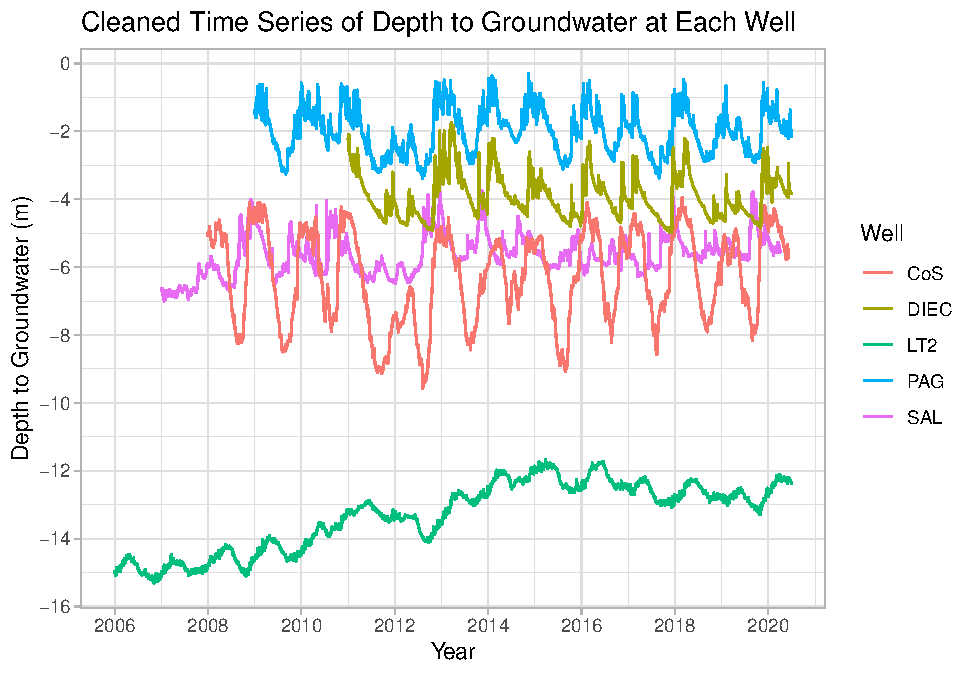
\includegraphics{Kaufman_McNeill_ENV797_Project_files/figure-latex/unnamed-chunk-3-2.pdf}

We followed the same process for the other variables (rainfall,
temperature, and volume) so that we had clean time series objects that
could be used as exogenous variables later on in the modeling and
forecasting portion of our process.

\begin{Shaded}
\begin{Highlighting}[]
\CommentTok{\#create a dataframe with date and rainfall data}
\NormalTok{auser\_rain }\OtherTok{\textless{}{-}}\NormalTok{ auser\_raw }\SpecialCharTok{\%\textgreater{}\%} 
  \FunctionTok{slice}\NormalTok{(}\DecValTok{2860}\SpecialCharTok{:}\DecValTok{8154}\NormalTok{) }\SpecialCharTok{\%\textgreater{}\%} 
  \FunctionTok{select}\NormalTok{(Date}\SpecialCharTok{:}\NormalTok{Rainfall\_Fabbriche\_di\_Vallico)}

\CommentTok{\#create a start date object for rainfall}
\NormalTok{start\_rain }\OtherTok{\textless{}{-}} \FunctionTok{as.Date}\NormalTok{(}\StringTok{"2006{-}01{-}01"}\NormalTok{)}

\CommentTok{\#find and print the row and column indices of NA values}
\NormalTok{na\_indices\_rain }\OtherTok{\textless{}{-}} \FunctionTok{which}\NormalTok{(}\FunctionTok{is.na}\NormalTok{(auser\_rain), }\AttributeTok{arr.ind =} \ConstantTok{TRUE}\NormalTok{)}
\FunctionTok{print}\NormalTok{(na\_indices\_rain)}
\end{Highlighting}
\end{Shaded}

\begin{verbatim}
##         row col
##   [1,] 2223   4
##   [2,] 2225   4
##   [3,] 2226   4
##   [4,] 2232   4
##   [5,] 2233   4
##   [6,] 2237   4
##   [7,] 1097   7
##   [8,] 1098   7
##   [9,] 1099   7
##  [10,] 1100   7
##  [11,] 1101   7
##  [12,] 1102   7
##  [13,] 1103   7
##  [14,] 1104   7
##  [15,] 1105   7
##  [16,] 1106   7
##  [17,] 1107   7
##  [18,] 1108   7
##  [19,] 1109   7
##  [20,] 1110   7
##  [21,] 1111   7
##  [22,] 1112   7
##  [23,] 1113   7
##  [24,] 1114   7
##  [25,] 1115   7
##  [26,] 1116   7
##  [27,] 1117   7
##  [28,] 1118   7
##  [29,] 1119   7
##  [30,] 1120   7
##  [31,] 1121   7
##  [32,] 1122   7
##  [33,] 1123   7
##  [34,] 1124   7
##  [35,] 1125   7
##  [36,] 1126   7
##  [37,] 1127   7
##  [38,] 1128   7
##  [39,] 1129   7
##  [40,] 1130   7
##  [41,] 1131   7
##  [42,] 1132   7
##  [43,] 1133   7
##  [44,] 1134   7
##  [45,] 1135   7
##  [46,] 1136   7
##  [47,] 1137   7
##  [48,] 1138   7
##  [49,] 1139   7
##  [50,] 1140   7
##  [51,] 1141   7
##  [52,] 1142   7
##  [53,] 1143   7
##  [54,] 1144   7
##  [55,] 1145   7
##  [56,] 1146   7
##  [57,] 1147   7
##  [58,] 1148   7
##  [59,] 1149   7
##  [60,] 1150   7
##  [61,] 1151   7
##  [62,] 1152   7
##  [63,] 1153   7
##  [64,] 1154   7
##  [65,] 1155   7
##  [66,] 1156   7
##  [67,] 1157   7
##  [68,] 1158   7
##  [69,] 1159   7
##  [70,] 1160   7
##  [71,] 1161   7
##  [72,] 1162   7
##  [73,] 1163   7
##  [74,] 1164   7
##  [75,] 1165   7
##  [76,] 1166   7
##  [77,] 1167   7
##  [78,] 1168   7
##  [79,] 1169   7
##  [80,] 1170   7
##  [81,] 1171   7
##  [82,] 1172   7
##  [83,] 1173   7
##  [84,] 1174   7
##  [85,] 1175   7
##  [86,] 1176   7
##  [87,] 1177   7
##  [88,] 1178   7
##  [89,] 1179   7
##  [90,] 1180   7
##  [91,] 1181   7
##  [92,] 1182   7
##  [93,] 1183   7
##  [94,] 1184   7
##  [95,] 1185   7
##  [96,] 1186   7
##  [97,] 1187   7
##  [98,] 1188   7
##  [99,] 1189   7
## [100,] 1190   7
## [101,] 1191   7
## [102,] 1192   7
## [103,] 1193   7
## [104,] 1194   7
## [105,] 1195   7
## [106,] 1196   7
## [107,] 1197   7
## [108,] 1198   7
## [109,] 1199   7
## [110,] 1200   7
## [111,] 1201   7
## [112,] 1202   7
## [113,] 1203   7
## [114,] 1204   7
## [115,] 1205   7
## [116,] 1206   7
## [117,] 1207   7
## [118,] 1208   7
## [119,] 1209   7
## [120,] 1210   7
## [121,] 1211   7
## [122,] 1212   7
## [123,] 1213   7
## [124,] 1214   7
## [125,] 1215   7
## [126,] 1216   7
## [127,] 1217   7
## [128,] 1218   7
## [129,] 1219   7
## [130,] 1220   7
## [131,] 1221   7
## [132,] 1222   7
## [133,] 1223   7
## [134,] 1224   7
## [135,] 1225   7
## [136,] 1226   7
## [137,] 1227   7
## [138,] 1228   7
## [139,] 1229   7
## [140,] 1230   7
## [141,] 1231   7
## [142,] 1232   7
## [143,] 1233   7
## [144,] 1234   7
## [145,] 1235   7
## [146,] 1236   7
## [147,] 1237   7
## [148,] 1238   7
## [149,] 1239   7
## [150,] 1240   7
## [151,] 1241   7
## [152,] 1242   7
## [153,] 1243   7
## [154,] 1244   7
## [155,] 1245   7
## [156,] 1246   7
## [157,] 1247   7
## [158,] 1248   7
## [159,] 1249   7
## [160,] 1250   7
## [161,] 1251   7
## [162,] 1252   7
## [163,] 1253   7
## [164,] 1254   7
## [165,] 1255   7
## [166,] 1256   7
## [167,] 1257   7
## [168,] 1258   7
## [169,] 1259   7
## [170,] 1260   7
## [171,] 1261   7
## [172,] 1262   7
## [173,] 1263   7
## [174,] 1264   7
## [175,] 1265   7
## [176,] 1266   7
## [177,] 1267   7
## [178,] 1268   7
## [179,] 1269   7
## [180,] 1270   7
## [181,] 1271   7
## [182,] 1272   7
## [183,] 1273   7
## [184,] 1274   7
## [185,] 1275   7
## [186,] 1276   7
## [187,] 1277   7
## [188,] 1278   7
## [189,] 1279   7
## [190,] 1280   7
## [191,] 1281   7
## [192,] 1282   7
## [193,] 1283   7
## [194,] 1284   7
## [195,] 1285   7
## [196,] 1286   7
## [197,] 1287   7
## [198,] 1288   7
## [199,] 1289   7
## [200,] 1290   7
## [201,] 1291   7
## [202,] 1292   7
## [203,] 1293   7
## [204,] 1294   7
## [205,] 1295   7
## [206,] 1296   7
## [207,] 1297   7
## [208,] 1298   7
## [209,] 1299   7
## [210,] 1300   7
## [211,] 1301   7
## [212,] 1302   7
## [213,] 1303   7
## [214,] 1304   7
## [215,] 1305   7
## [216,] 1306   7
## [217,] 1307   7
## [218,] 1308   7
## [219,] 1309   7
## [220,] 1310   7
## [221,] 1311   7
## [222,] 1312   7
## [223,] 1313   7
## [224,] 1314   7
## [225,] 1315   7
## [226,] 1316   7
## [227,] 1317   7
## [228,] 1318   7
## [229,] 1319   7
## [230,] 1320   7
## [231,] 1321   7
## [232,] 1322   7
## [233,] 1323   7
## [234,] 1324   7
## [235,] 1325   7
## [236,] 1326   7
## [237,] 1327   7
## [238,] 1328   7
## [239,] 1329   7
## [240,] 1330   7
## [241,] 1331   7
## [242,] 1332   7
## [243,] 1333   7
## [244,] 1334   7
## [245,] 1335   7
## [246,] 1336   7
## [247,] 1337   7
## [248,] 1338   7
## [249,] 1339   7
## [250,] 1340   7
## [251,] 1341   7
## [252,] 1342   7
## [253,] 1343   7
## [254,] 1344   7
## [255,] 1345   7
## [256,] 1346   7
## [257,] 1347   7
## [258,] 1348   7
## [259,] 1349   7
## [260,] 1350   7
## [261,] 1351   7
## [262,] 1352   7
## [263,] 1353   7
## [264,] 1354   7
## [265,] 1355   7
## [266,] 1356   7
## [267,] 1357   7
## [268,] 1358   7
## [269,] 1359   7
## [270,] 1360   7
## [271,] 1361   7
## [272,] 1362   7
## [273,] 1363   7
## [274,] 1364   7
## [275,] 1365   7
## [276,] 1366   7
## [277,] 1367   7
## [278,] 1368   7
## [279,] 1369   7
## [280,] 1370   7
## [281,] 1371   7
## [282,] 1372   7
## [283,] 1373   7
## [284,] 1374   7
## [285,] 1375   7
## [286,] 1376   7
## [287,] 1377   7
## [288,] 1378   7
## [289,] 1379   7
## [290,] 1380   7
## [291,] 1381   7
## [292,] 1382   7
## [293,] 1383   7
## [294,] 1384   7
## [295,] 1385   7
## [296,] 1386   7
## [297,] 1387   7
## [298,] 1388   7
## [299,] 1389   7
## [300,] 1390   7
## [301,] 1391   7
## [302,] 1392   7
## [303,] 1393   7
## [304,] 1394   7
## [305,] 1395   7
## [306,] 1396   7
## [307,] 1397   7
## [308,] 1398   7
## [309,] 1399   7
## [310,] 1400   7
## [311,] 1401   7
## [312,] 1402   7
## [313,] 1403   7
## [314,] 1404   7
## [315,] 1405   7
## [316,] 1406   7
## [317,] 1407   7
## [318,] 1408   7
## [319,] 1409   7
## [320,] 1410   7
## [321,] 1411   7
## [322,] 1412   7
## [323,] 1413   7
## [324,] 1414   7
## [325,] 1415   7
## [326,] 1416   7
## [327,] 1417   7
## [328,] 1418   7
## [329,] 1419   7
## [330,] 1420   7
## [331,] 1421   7
## [332,] 1422   7
## [333,] 1423   7
## [334,] 1424   7
## [335,] 1425   7
## [336,] 1426   7
## [337,] 1427   7
## [338,] 1428   7
## [339,] 1429   7
## [340,] 1430   7
## [341,] 1431   7
## [342,] 1432   7
## [343,] 1433   7
## [344,] 1434   7
## [345,] 1435   7
## [346,] 1436   7
## [347,] 1437   7
## [348,] 1438   7
## [349,] 1439   7
## [350,] 1440   7
## [351,] 1441   7
## [352,] 1442   7
## [353,] 1443   7
## [354,] 1444   7
## [355,] 1445   7
## [356,] 1446   7
## [357,] 1447   7
## [358,] 1448   7
## [359,] 1449   7
## [360,] 1450   7
## [361,] 1451   7
## [362,] 1452   7
## [363,] 1453   7
## [364,] 1454   7
## [365,] 1455   7
## [366,] 1456   7
## [367,] 1457   7
## [368,] 1458   7
## [369,] 1459   7
## [370,] 1460   7
## [371,] 1461   7
\end{verbatim}

\begin{Shaded}
\begin{Highlighting}[]
\CommentTok{\#plotting rainfall, need to fill in na and then make TS}
\FunctionTok{ggplot}\NormalTok{(auser\_rain)}\SpecialCharTok{+} 
  \FunctionTok{geom\_line}\NormalTok{(}\FunctionTok{aes}\NormalTok{(}\AttributeTok{x=}\NormalTok{Date, }\AttributeTok{y=}\NormalTok{Rainfall\_Fabbriche\_di\_Vallico))}
\end{Highlighting}
\end{Shaded}

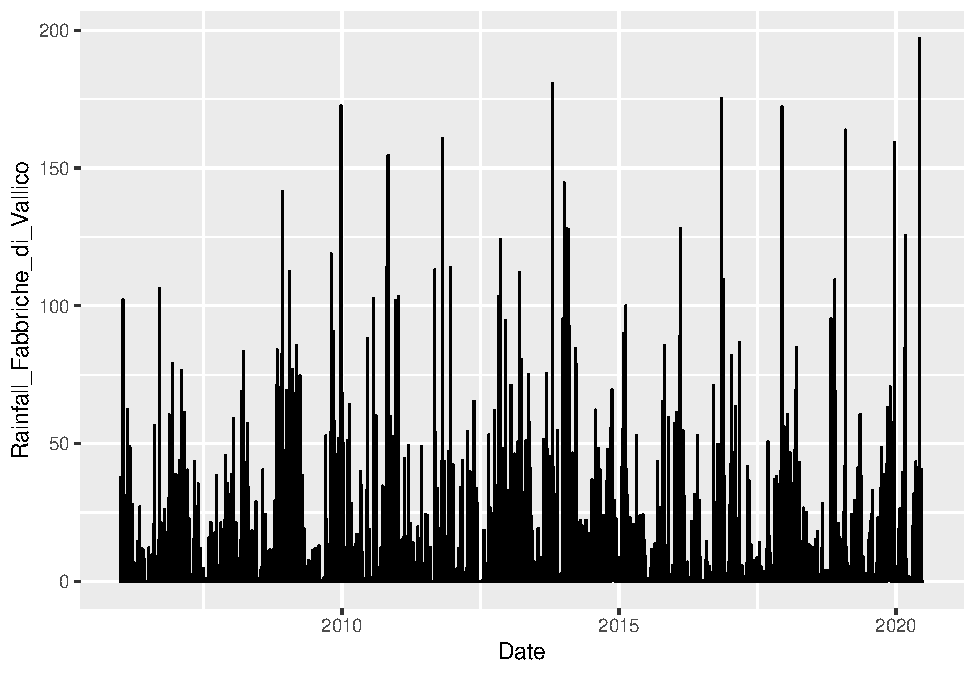
\includegraphics{Kaufman_McNeill_ENV797_Project_files/figure-latex/unnamed-chunk-4-1.pdf}

\begin{Shaded}
\begin{Highlighting}[]
\NormalTok{ts\_rain }\OtherTok{\textless{}{-}} \FunctionTok{ts}\NormalTok{(auser\_rain[,}\DecValTok{2}\SpecialCharTok{:}\DecValTok{11}\NormalTok{],}\AttributeTok{start=}\FunctionTok{c}\NormalTok{(}\DecValTok{2006}\NormalTok{,}\DecValTok{01}\NormalTok{,}\DecValTok{01}\NormalTok{), }\AttributeTok{frequency=}\DecValTok{365}\NormalTok{)}

\FunctionTok{autoplot}\NormalTok{(ts\_rain)}
\end{Highlighting}
\end{Shaded}

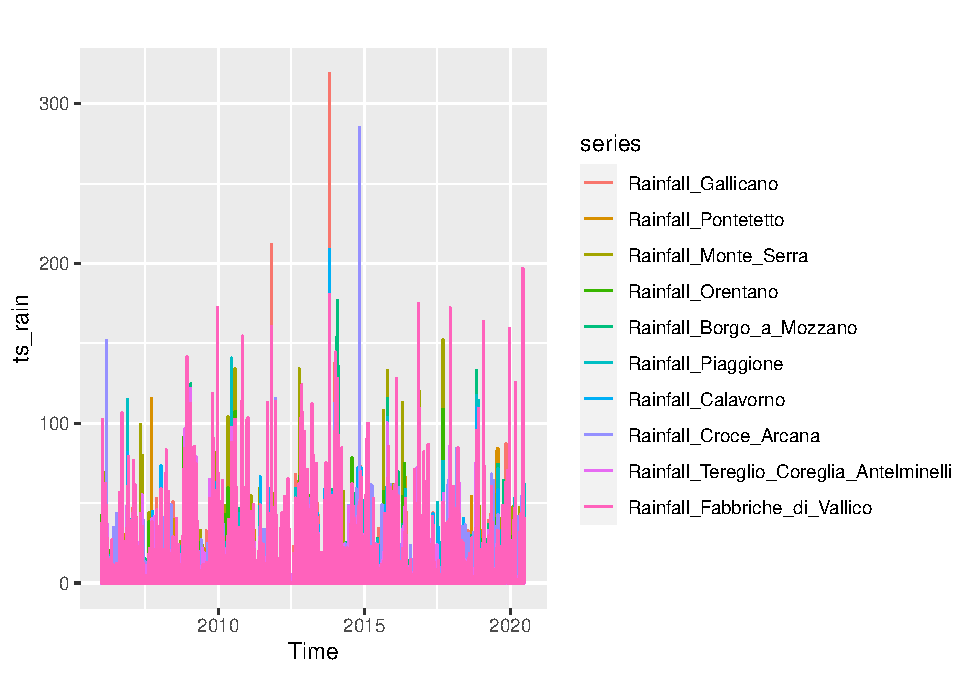
\includegraphics{Kaufman_McNeill_ENV797_Project_files/figure-latex/unnamed-chunk-4-2.pdf}

\begin{Shaded}
\begin{Highlighting}[]
\CommentTok{\#to do: make a timeseries object that has interpolated na values? }
\end{Highlighting}
\end{Shaded}

\begin{Shaded}
\begin{Highlighting}[]
\CommentTok{\#create a dataframe with date and temperature data}
\NormalTok{auser\_temp }\OtherTok{\textless{}{-}}\NormalTok{ auser\_raw }\SpecialCharTok{\%\textgreater{}\%} 
  \FunctionTok{select}\NormalTok{(Date,Temperature\_Orentano}\SpecialCharTok{:}\NormalTok{Temperature\_Lucca\_Orto\_Botanico)}

\CommentTok{\#create a start date object for temperature}
\NormalTok{start\_temp }\OtherTok{\textless{}{-}} \FunctionTok{as.Date}\NormalTok{(}\StringTok{"1998{-}03{-}05"}\NormalTok{)}

\CommentTok{\#note: 0 is essentially NA for the beginning rows, true zero is 0.0}
\end{Highlighting}
\end{Shaded}

\begin{Shaded}
\begin{Highlighting}[]
\CommentTok{\#create a dataframe with date and volume data}
\NormalTok{auser\_volume }\OtherTok{\textless{}{-}}\NormalTok{ auser\_raw }\SpecialCharTok{\%\textgreater{}\%} 
  \FunctionTok{slice}\NormalTok{(}\DecValTok{2495}\SpecialCharTok{:}\DecValTok{8154}\NormalTok{) }\SpecialCharTok{\%\textgreater{}\%} 
  \FunctionTok{select}\NormalTok{(Date,Volume\_POL}\SpecialCharTok{:}\NormalTok{Volume\_CSAL)}

\CommentTok{\#create a start date object for volume}
\NormalTok{start\_volume }\OtherTok{\textless{}{-}} \FunctionTok{as.Date}\NormalTok{(}\StringTok{"2005{-}01{-}01"}\NormalTok{)}
\end{Highlighting}
\end{Shaded}

The last bit of data wrangling that we performed was running the
correlation function on our groundwater data to discern whether the
depth to groundwater values at the five wells were correlated to one
another. We found that the four north wells had similar correlation
values to one another and that the one south well was weakly correlated
to the others. Our correlation plot

\begin{Shaded}
\begin{Highlighting}[]
\CommentTok{\#looking at initial correlation of groundwater wells}
\NormalTok{auser\_subset }\OtherTok{\textless{}{-}}\NormalTok{ auser\_raw }\SpecialCharTok{\%\textgreater{}\%}
  \FunctionTok{rename}\NormalTok{(}\AttributeTok{LT2 =}\NormalTok{ Depth\_to\_Groundwater\_LT2,}
         \AttributeTok{SAL =}\NormalTok{ Depth\_to\_Groundwater\_SAL,}
         \AttributeTok{PAG =}\NormalTok{ Depth\_to\_Groundwater\_PAG,}
         \AttributeTok{CoS =}\NormalTok{ Depth\_to\_Groundwater\_CoS,}
         \AttributeTok{DIEC =}\NormalTok{ Depth\_to\_Groundwater\_DIEC) }\SpecialCharTok{\%\textgreater{}\%}
  \FunctionTok{select}\NormalTok{(LT2}\SpecialCharTok{:}\NormalTok{DIEC) }\SpecialCharTok{\%\textgreater{}\%}
  \FunctionTok{na.omit}\NormalTok{()}

\CommentTok{\#how correlated are the different groundwater wells within one aquifer?}
\NormalTok{auser\_correlation }\OtherTok{\textless{}{-}} \FunctionTok{cor}\NormalTok{(auser\_subset)}
\FunctionTok{corrplot}\NormalTok{(auser\_correlation, }\AttributeTok{method =} \StringTok{"ellipse"}\NormalTok{)}
\end{Highlighting}
\end{Shaded}

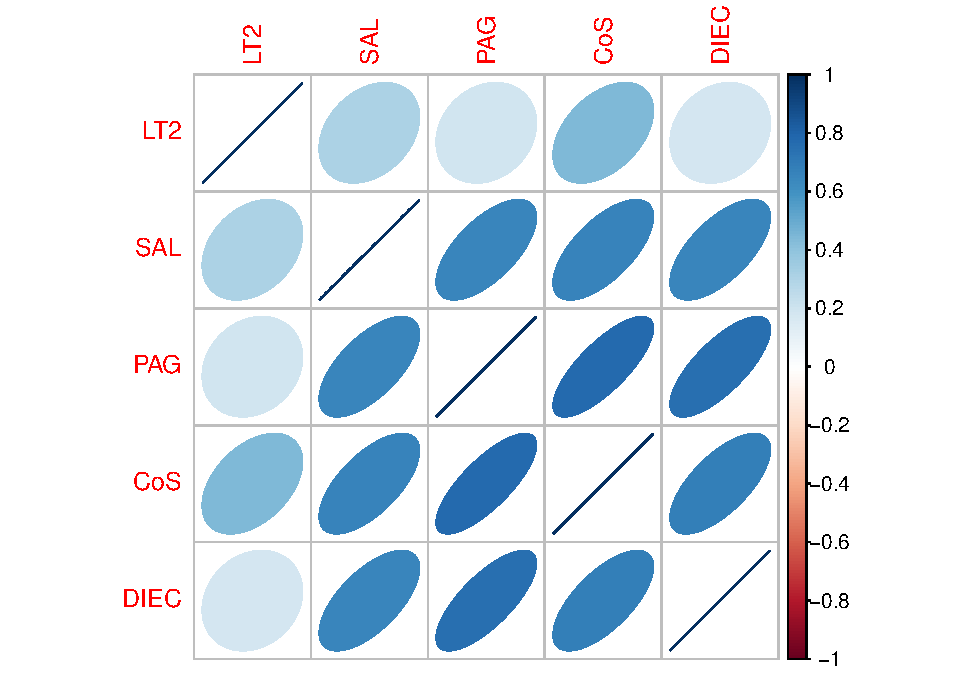
\includegraphics{Kaufman_McNeill_ENV797_Project_files/figure-latex/correlation plots-1.pdf}

\begin{Shaded}
\begin{Highlighting}[]
\FunctionTok{corrplot.mixed}\NormalTok{(auser\_correlation, }\AttributeTok{upper =} \StringTok{"ellipse"}\NormalTok{)}
\end{Highlighting}
\end{Shaded}

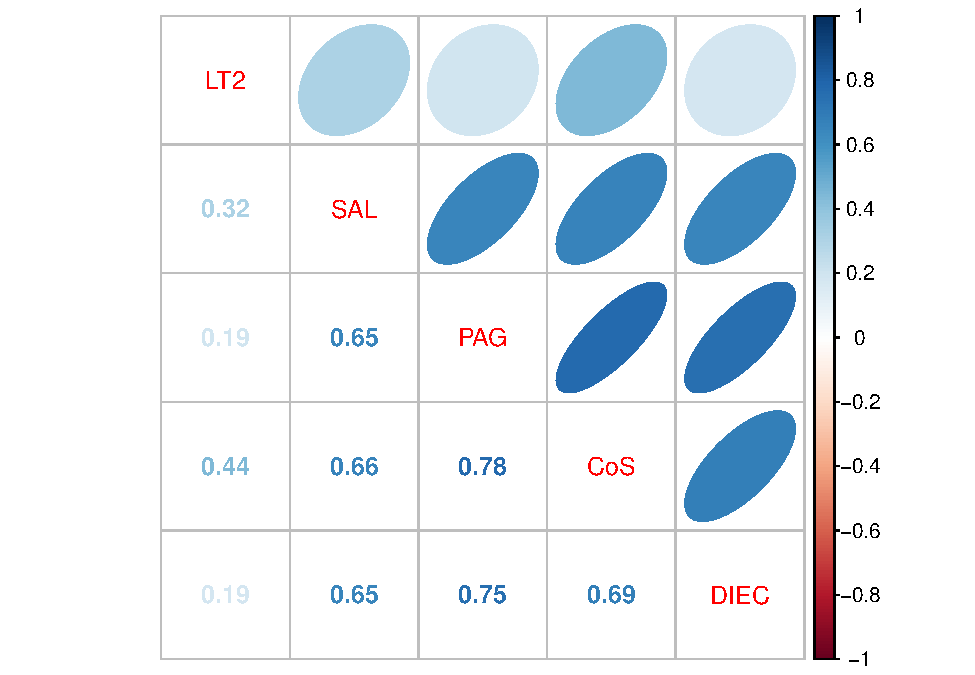
\includegraphics{Kaufman_McNeill_ENV797_Project_files/figure-latex/correlation plots-2.pdf}

\end{document}
